\documentclass[12pt] {article}
\usepackage{times}
\usepackage[margin=0.6in,bottom=1in,top=0.5in]{geometry}

\usepackage{hhline}
\usepackage{subfig}
\usepackage{graphicx}
\usepackage{amsmath}




\begin{document}

\title{Graph Coloring -  EEC289Q}
\author{Yuxin Chen and Ahmed H. Mahmoud}
\date{February 22nd, 2018}
\maketitle
%============Table========
%\begin{figure}[tbh]
% \centering    
%\begin{tabular}{ |p{4cm}|| p{2cm}|p{2cm}|p{2cm}|p{2cm}|}
% \hline
% & Processor 1 &  Processor 2  & Processor 3 & Processor 4\\ \hhline{|=|=|=|=|=|}
% \hline
% Performance          &$1.08$        &$1.425$       &\textbf{1.52}  &   \\
% \hline
%\end{tabular} 
%\caption{Metric table for the four processors}
%   \label{tab:metric}
%\end{figure} 
%============Figure========
%\begin{figure}[!tbh]
%\centering        
%   \subfloat {\includegraphics[width=0.65\textwidth]{fig2_4.png}}
%   \caption{ }
%   \label{fig:fig}
%\end{figure}

\section{Algorithm Details:}
Generally, there are two approach to do graph coloring: 1) independent set based 2) greedy algrithm based. In our work, we chose to use independent set based algorithm. Basically we generate each node a random number, and for each node, it can be added to the current independent set only if it has the maxinum random number among its neighbors. So this method ensure every node within the same independent set, they are not connected since they can not be maxinum at the same time. Next iteraion we find the maxinum vertex on nodes left (exclude nodes which are in the independent sets) and form a new indepedent set. The algorithm continues untill all the nodes belong to independent sets.

\subsection{An naive implementation}
An naive implementation: 
\begin{figure}[!tbh]
\centering        
   \subfloat[lol] {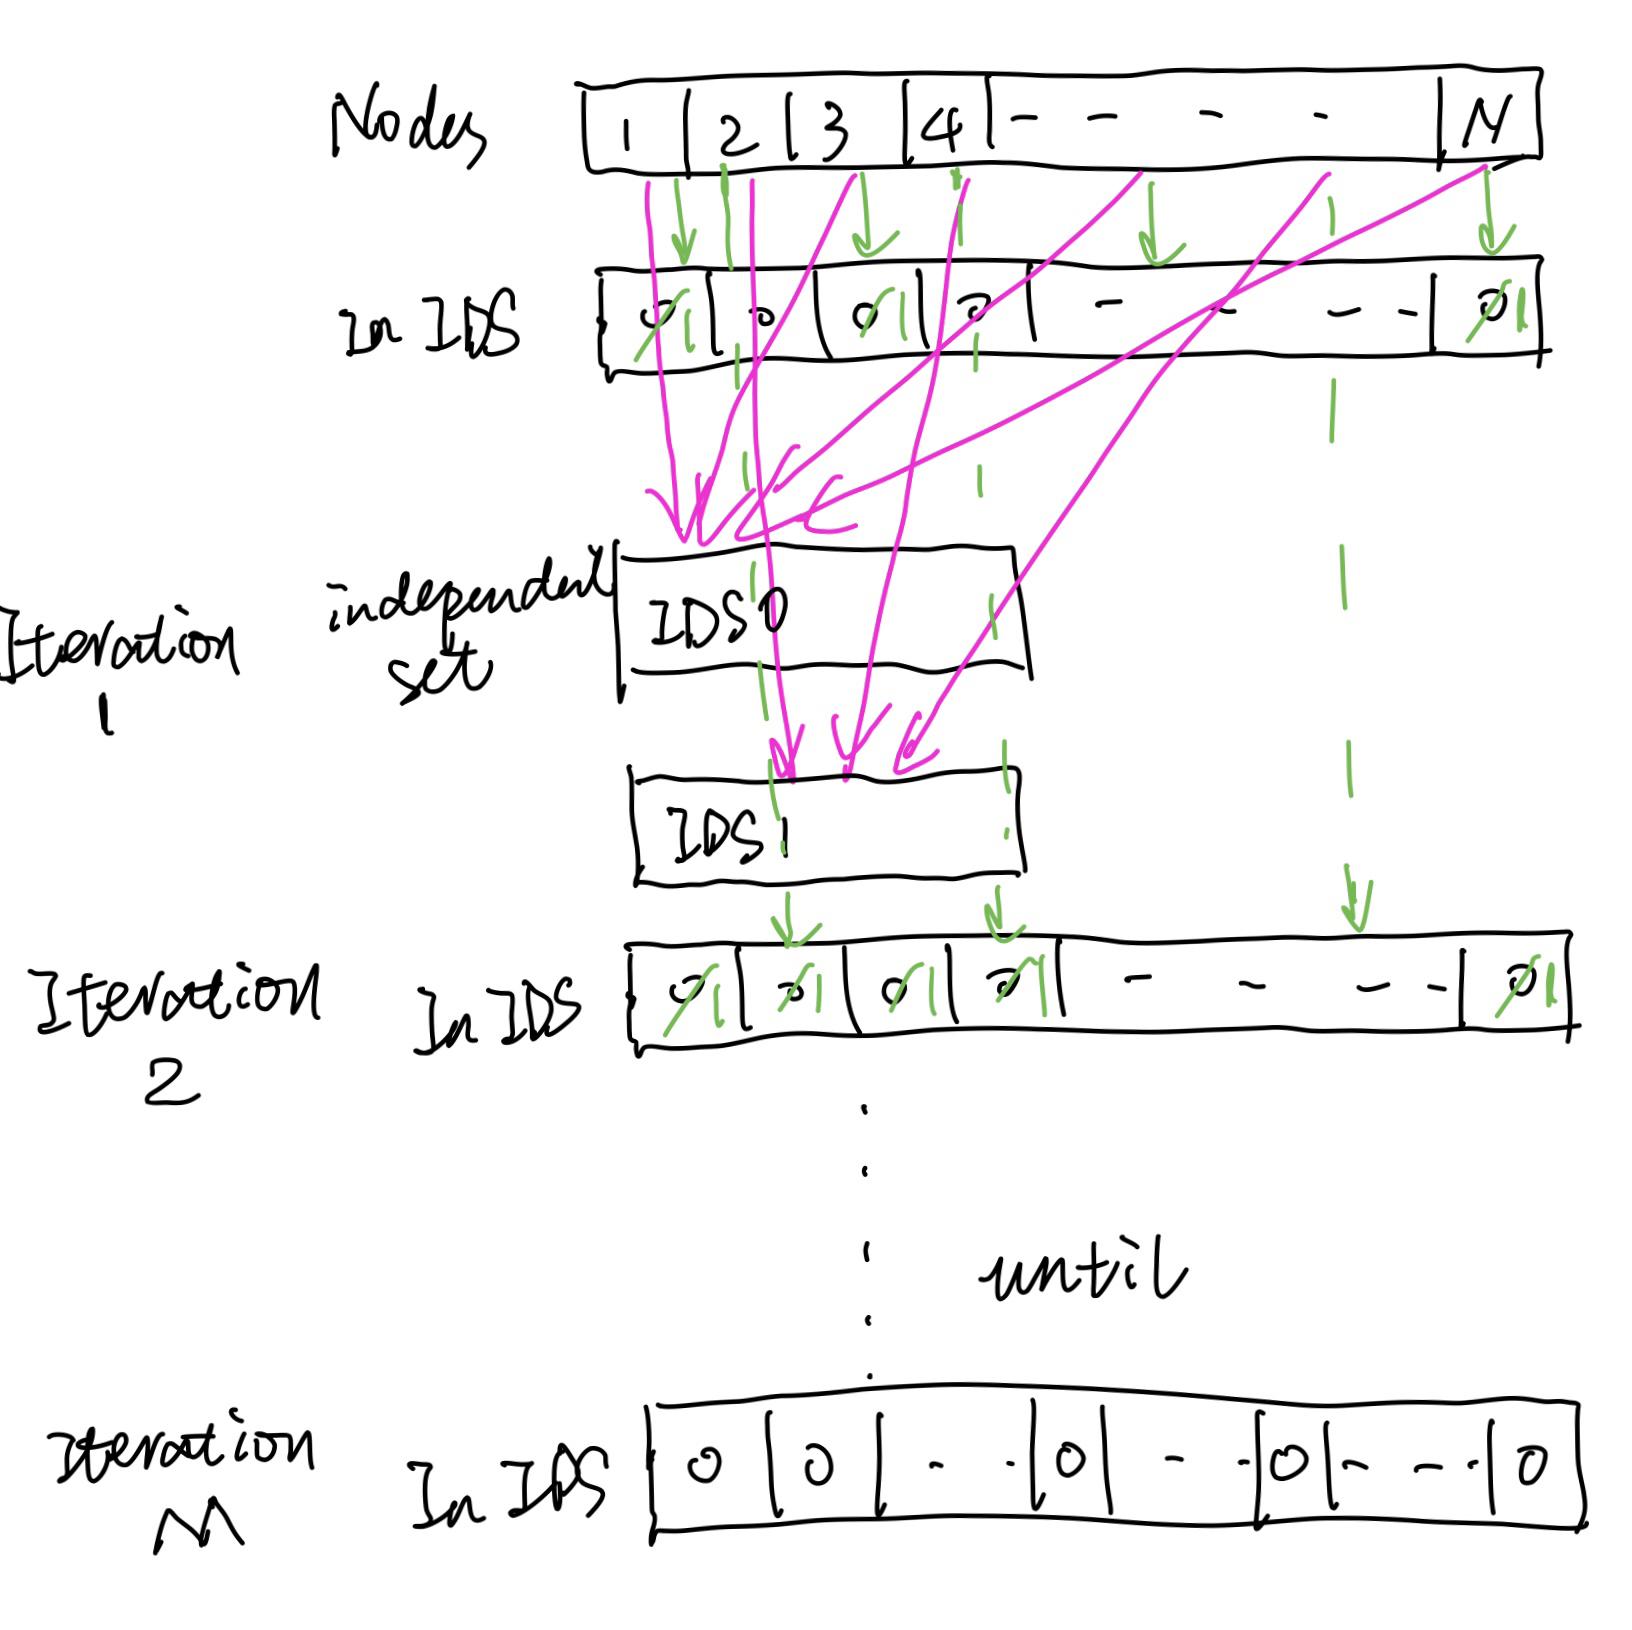
\includegraphics[width=0.24\textwidth]{naive.jpg}}
   \subfloat[lol1] {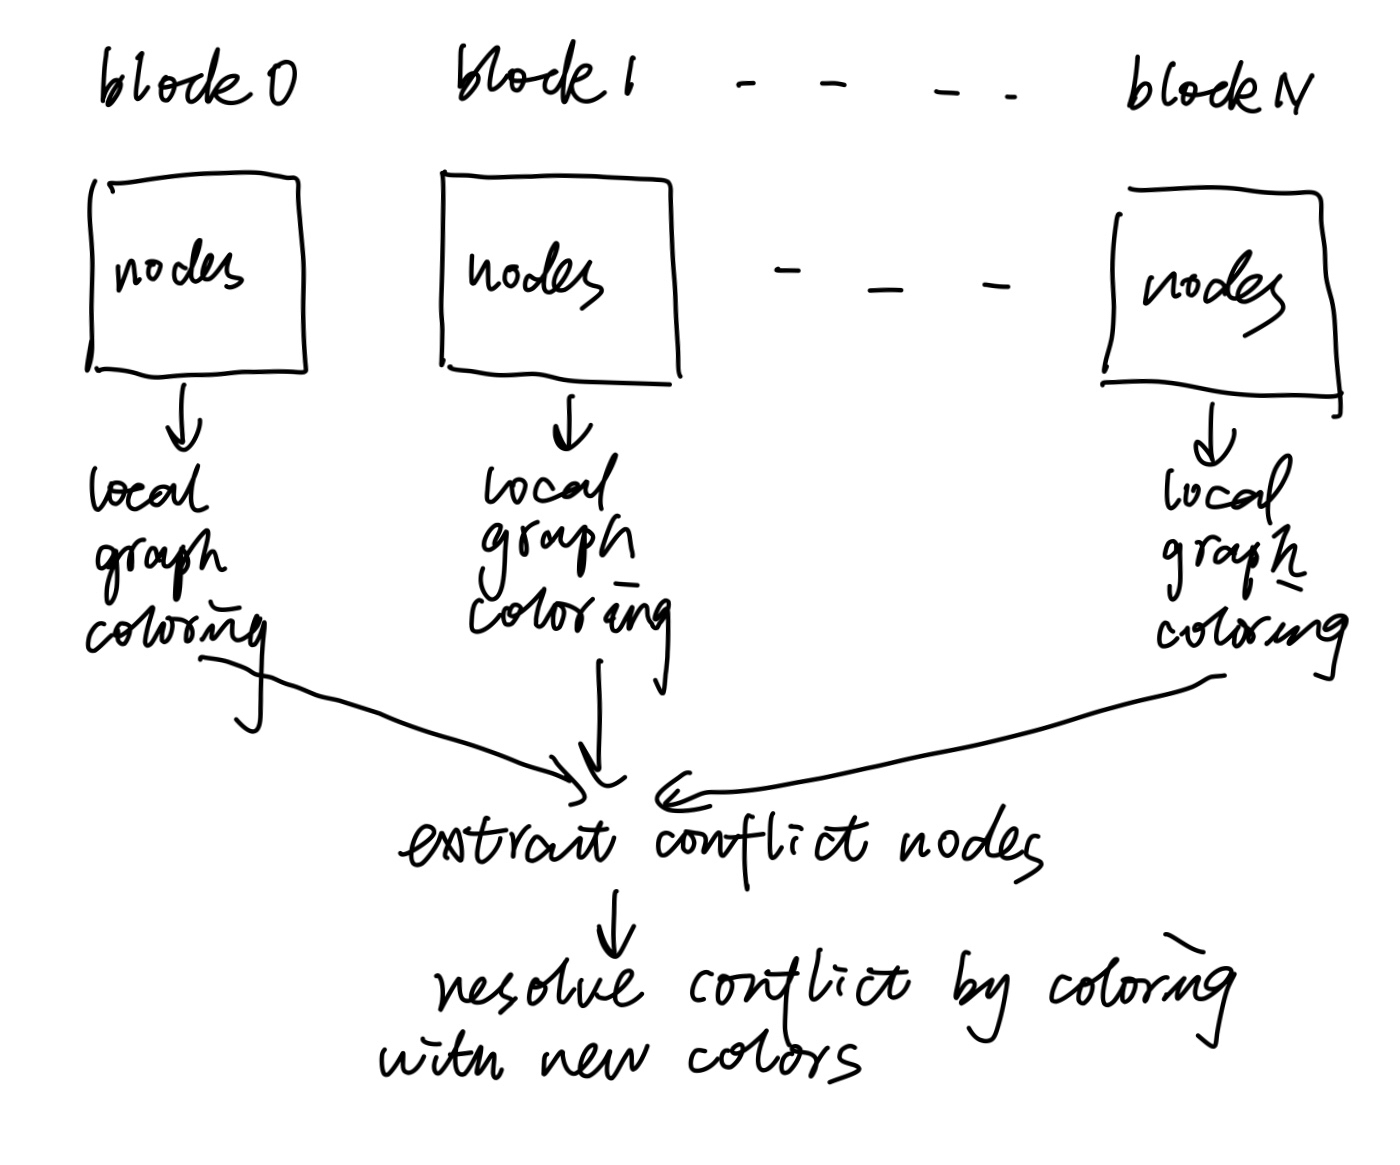
\includegraphics[width=0.24\textwidth]{comfree.jpg}}
   \subfloat[] {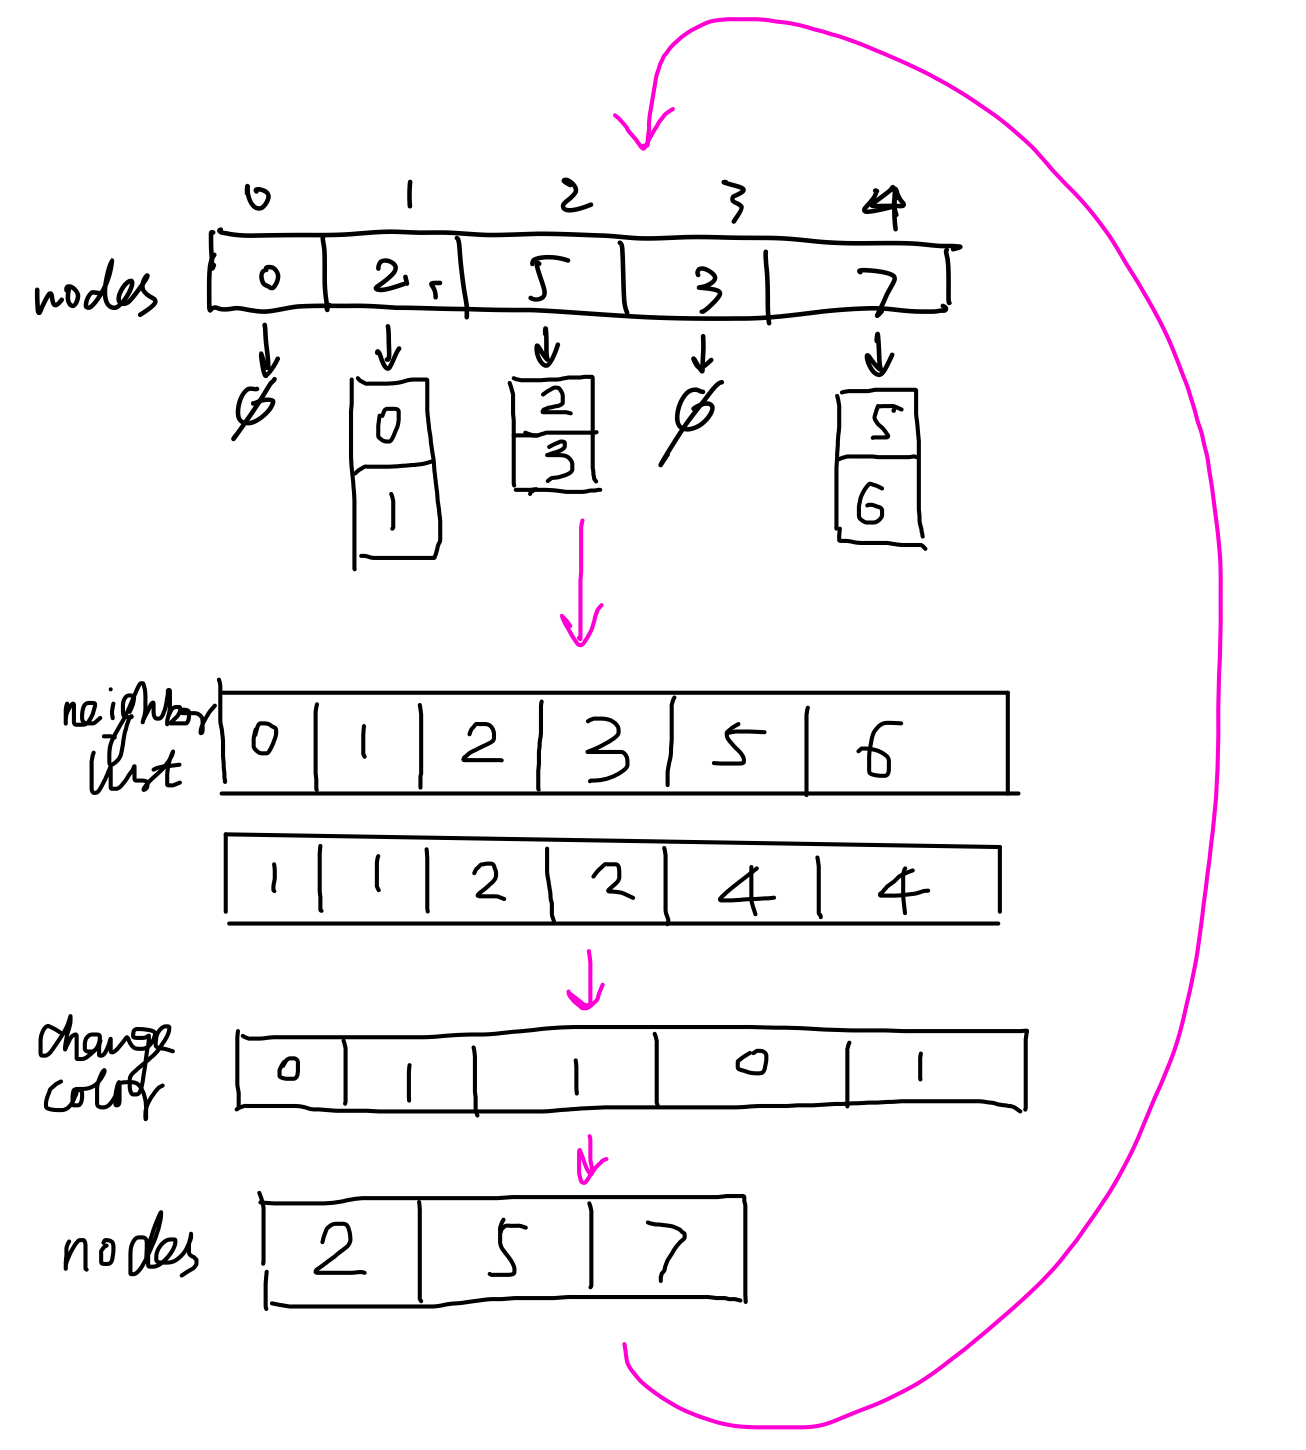
\includegraphics[width=0.24\textwidth]{confre.jpg}}
   \subfloat[] {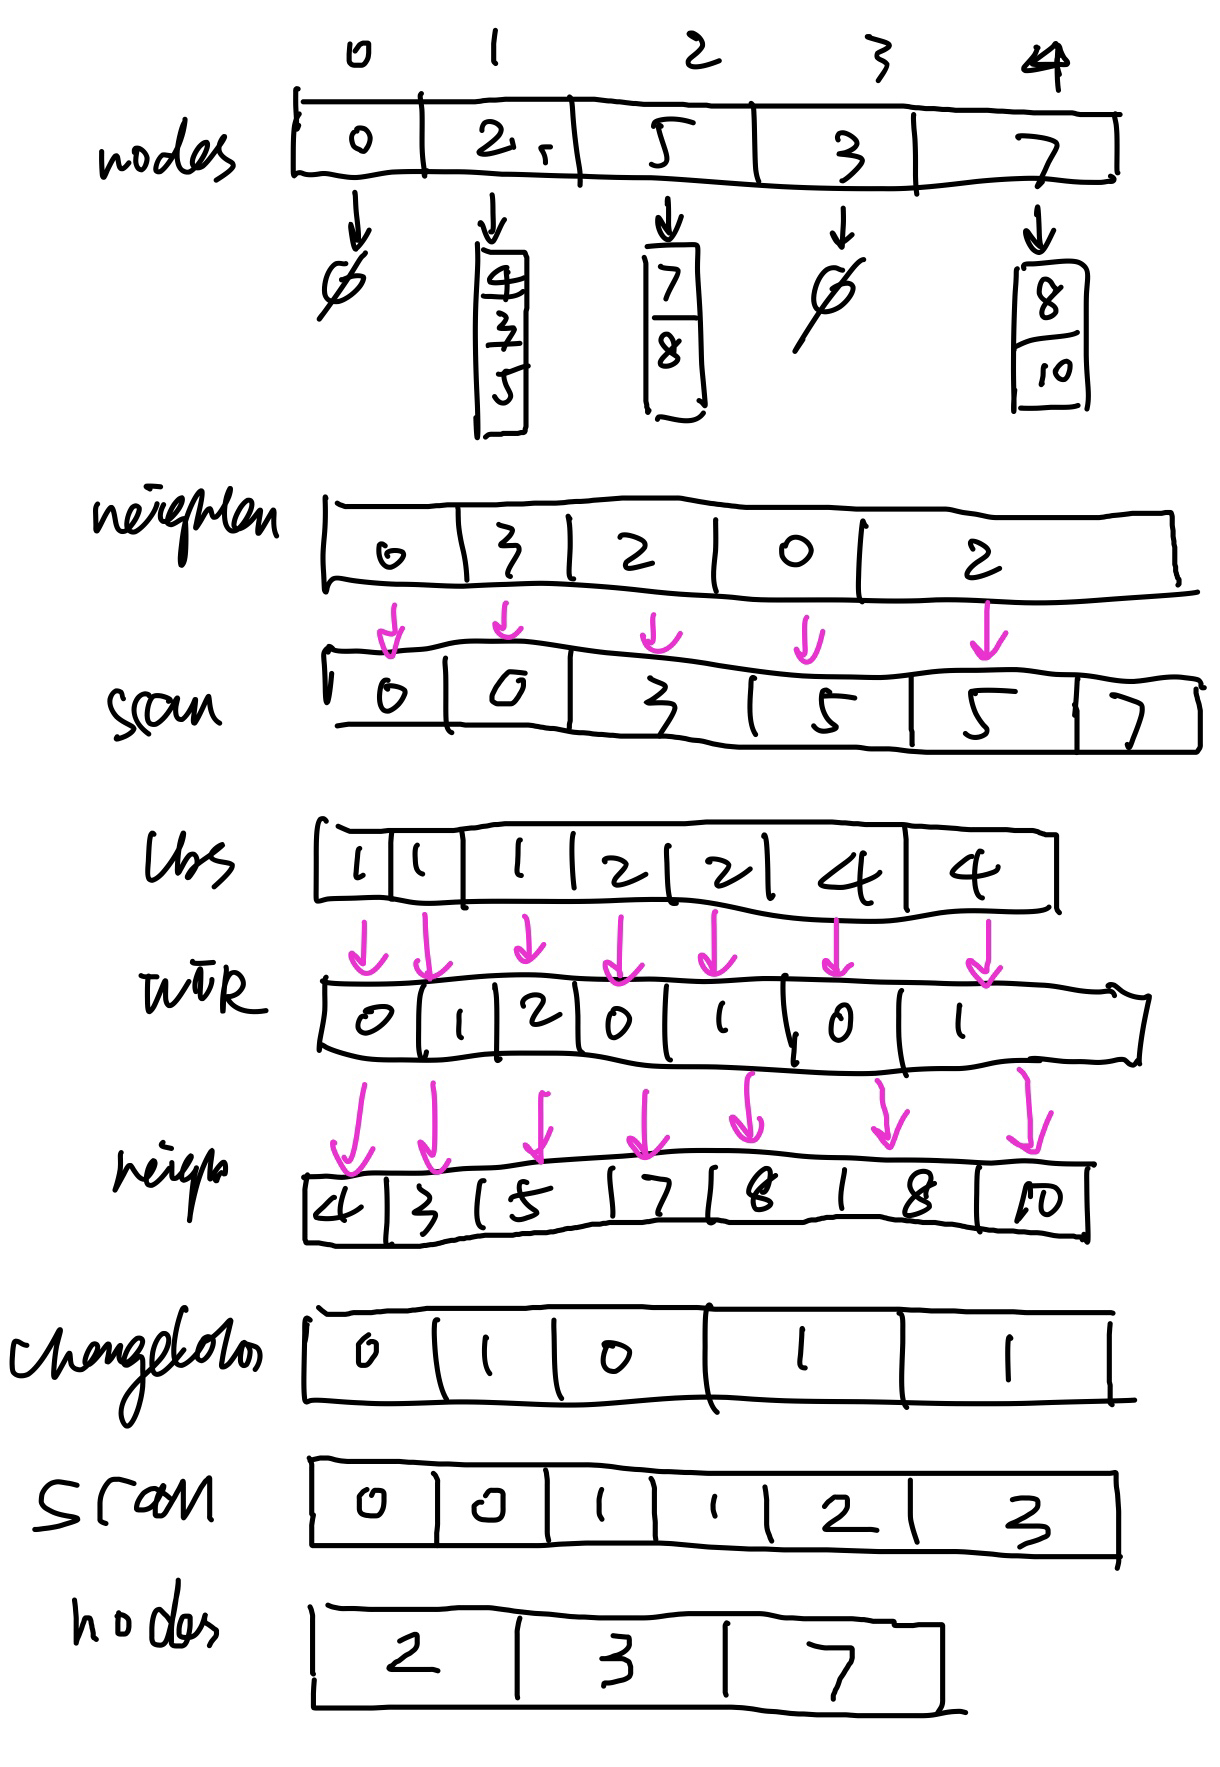
\includegraphics[width=0.24\textwidth]{scanlbswir.jpg}}
   \caption{ }
   \label{fig:fig1}
\end{figure}

Each iteration, each thread access one node, it will see first if its InIDS value is 1, if yes, it exits, if no, it needs to see its neighbor's InIDS value and only compares the node's random number with its neighbors's whose InIDS value is 0. If it is the maxinum among its neighbors, it first writes itself into independent set IDS0 (or IDS1, IDS2, depdent on the iteration), and set the node's InIDS value to 1. Then it goes to next iteration. 

So if at this iteration, a node is not included into an independent set, next iteration, it still needs to compare with its live neighbors (dead if some node are included in an independent set). This node will keep using the same neighbor list until it is added to an independent set. There is potential two improvement for this naive implementation: 1) since some thread will access node who are in independent sets, then exits imediatly. Since threads are executed in warps, if half of the threads in a warp exit imediately, then we wasting computing cycles and unter utilize the hardware. 2) There are data reuse. Now all the memory access goes through global memory. We should think about using shared memory.

Now just think about how to use shared memroy, if we distributed nodes to different blocks, each node can load its neighbor list into shared memory and reuse it until it is added to an independent set. However, each iteration, the node also needs to know its neighbor's status (if added to IDS). If its neighbor belongs to other block, it is hard to keep data coherency among blocks. 

\subsection{Communication free graph coloring}
We propose this communication free graph coloring approach:
\begin{figure}[!tbh]
\centering        
   \subfloat {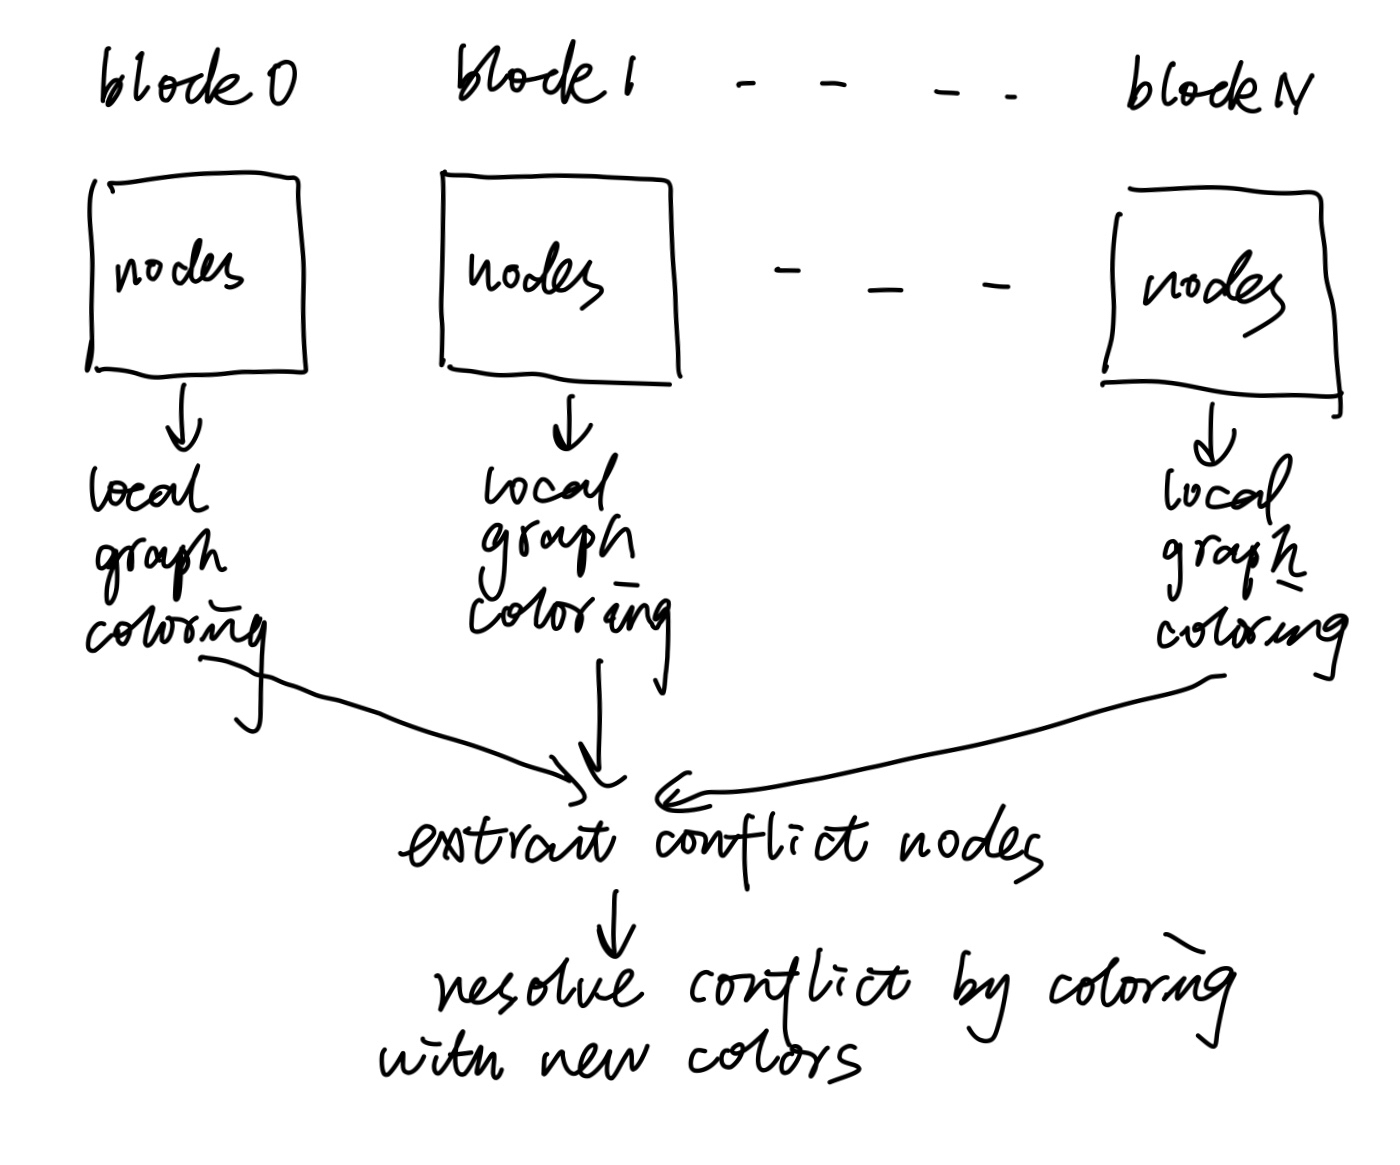
\includegraphics[width=0.3\textwidth]{comfree.jpg}}
   \caption{ }
   \label{fig:fig2}
\end{figure} 

When we run local graph coloring, we use the algorithm we describe above and ignoring the nodes's neighbors who are on other blocks, i.e we don't exame the neighbor who belongs to other blocks. After each block finishs local graph coloring, the conflict can only happen between nodes who belong to different blocks. Then we extract those nodes only and form a new conflict graph and resolve those conflict by assigning new colors. We are expecting, in pratices, the conflict graph would be small and the number of colors used in local graph coloring will not bad. Because we run local graph coloring in shared memory, it should be fast. 

\section{Implementation:}

\subsection{Local graph coloring}

\subsection{Conflict resolve}
After the steps above, we have the conflict graph which is a format of CSR grouped by color. We process each color in sequence. We can definitely process all the color generated in previous step in parallel and each block will get one color, so there is a load balancing problem and we don't have time to do that. 

Give an array of conflict nodes of same color, we resolve the conflict by finding the neighbors of each node who have the same color and comparing the node ID with its conflict neighbor's ID, the one with lower ID will not change color, the one with higher ID will assigne a new color. For example nodes [1,2,3,4] are conflict nodes whose color is red. node 1 connects to node 3, node 2 connects to node 4. Then we run the algorithm, node 1 will find node 3 is its neighbor, but node 3's ID is higher, then, node 1 will not change its color. Node 3 will find node 1 is its neighbor, and node 1's ID is lower than its ID, then, node 3 will change its color to a new color purple. Some thing for node 2 and node 4, node 2 will not change its color and node 4 will change its color to new color purple. Then we need to review those nodes who assign new color again to ensure they are not conflict to each other. Then we find out node 3's neighbor, and find out node 3 doesn't have conflict neighbors, and for node 4, find out node 4 doesn't have conflict neighbors. Then the conflict nodes originally in color red now are resolved. If node 3 and node 4 are connected, then, we will find out node 3 won't change color since it has lower ID and node 4 will be assigned a new color yellow. We will need to review all the changed color nodes again which is node 4 and find out node 4 doesn't have conflict and all the conflict resolved. 

We do the above process for each color sequentially. After that, we can resolve all the conflict. 

There are some implementation optimization:
\begin{itemize}
\item When we get a node and need to find out its neighbor, since the neighbor whose ID is higher than the node, we won't change the node's color. We should not exam its neighbor whose ID is higher. We can acchive this by just using the lower triangle of the graph adjacency matrix. 

\item What we start with is an array of conflict nodes.

\begin{figure}[!tbh]
\centering        
   \subfloat {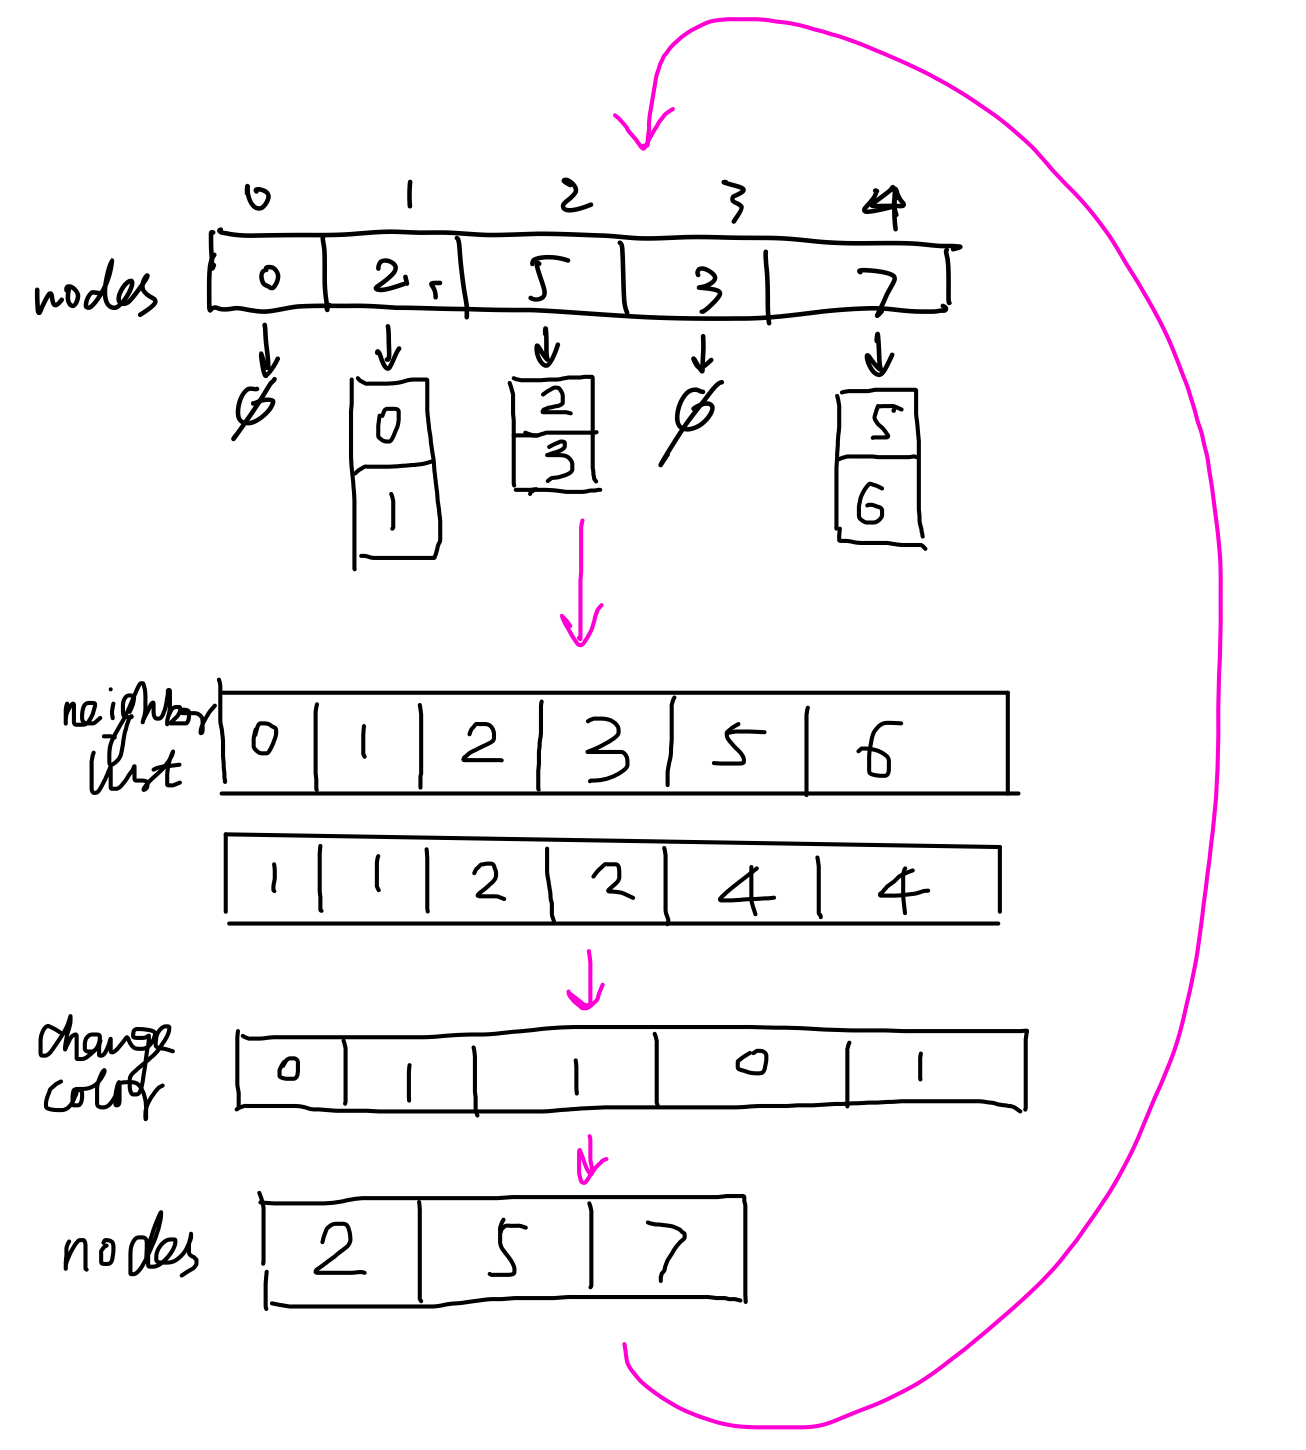
\includegraphics[width=0.3\textwidth]{confre.jpg}}
   \caption{ }
   \label{fig:fig3}
\end{figure} 

We want to get each node's neighbor list to tell if we need change this nodes' color. However if we map each thread to a node in the node array and read its neighbor list and seeif the node need change color, we will have very unbalanced work load for each thread, since the neighbor list for each node can vary a lot, then we are wasting computing cycle waiting for the thread who works on the longest neighbor list. We would prefer each thread work on each neighbor of each node. To have enough information to acchieve this mapping, we need to do extra work:
\begin{figure}[!tbh]
\centering        
   \subfloat {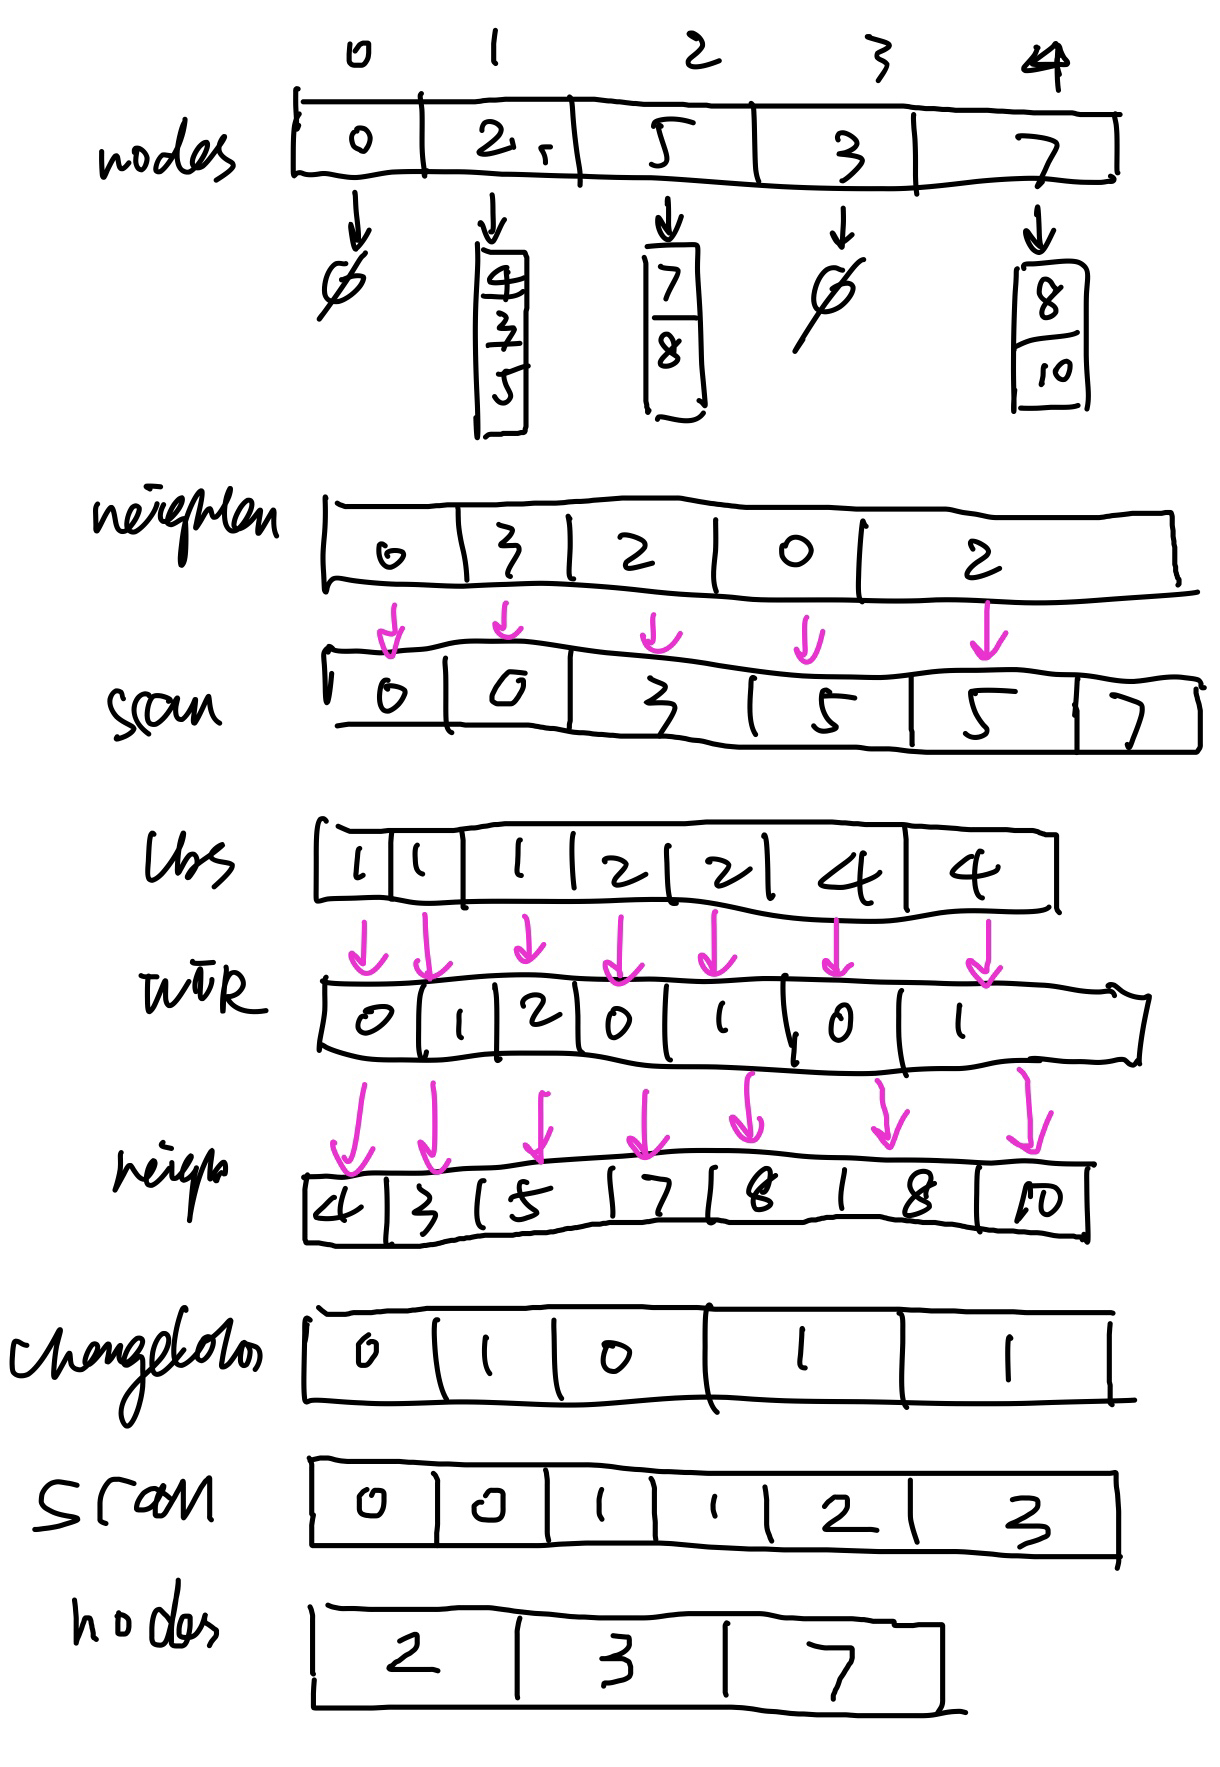
\includegraphics[width=0.3\textwidth]{scanlbswir.jpg}}
   \caption{ }
   \label{fig:fig4}
\end{figure} 

First we ask each thread to load a neighbor of a node and save it in register. To do this, each thread need to know which node's neighbor list, and the position of that neighbor in that neighbor list. To compute which node's neighbor list each thread need to access, we fist compute neighlen array by each thread get the neighbor list's length of each node, then we do scan on neighlen and compute load balancing search on the scan result. To compute the postion each thread should access in assigned neighbor list, we compute the work item rank (wir) array by computing $lbs[i]=i-scan[lbs[i]]$. After this, each thread can access each neighbor just using $tr\_col\_id[tr\_offset[nodes[lbs[i]]] + wir[i]]$, where $tr\_col\_id$ is the CSR column ID array for the conflict graph and $tr\_offset$ is the CSR row offset array for the conflict graph. Now we can exam the neighbor's color and produce a predicate array of if change color. Using this changeColor array, we can assign new color to nodes who need change color and do scan on changeColor, we can compact those nodes who need change color into a new array. Then go back to the top of the loop until there is no node who need to change color.

\end{itemize}

\section{Other approach}
Another good approach is to distribute nodes to different blocks and generate a random number each iteration and synchronize all the blocks using cooperative group in CUDA 9 or above. Then we can keep the neighbor list in the share memory all the time. One consideration is it is better for each node have a different random number otherwise it will increase the number of iteration to finish coloring. If we set the random number range large enough, the probability to get same random number for different nodes is very low.

\end{document}
